\documentclass{article}

\usepackage{tikz}

\begin{document}

    \begin{center}
        \Huge
        Quadrifolium curves
        \normalsize

        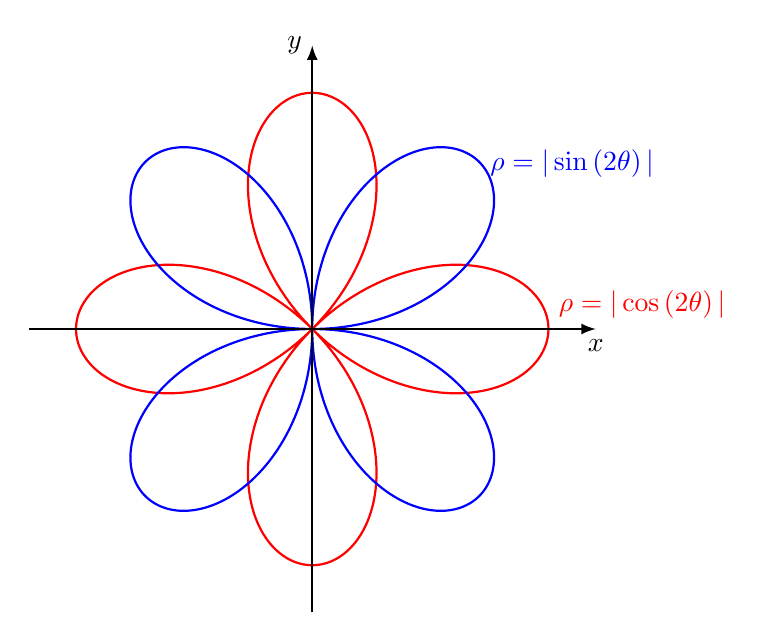
\begin{tikzpicture}[scale=3]
            \draw[color=red, thick, domain=0:360,smooth,variable=\t, samples=300] 
            plot ({\t}:{abs(cos(2*\t))}) node[above right] {\(\rho=|\cos\left(2\theta\right)|\)};
    
            \draw[color=blue, thick, domain=0:360,smooth,variable=\t, samples=300] 
                plot ({\t}:{abs(sin(2*\t))});
            \node[color=blue] at (1.1,0.7){\(\rho=|\sin\left(2\theta\right)|\)};
    
            \draw[thick, ->, >=latex] (-1.2,0) -- (1.2,0) node[below]{\(x\)};
            \draw[thick, ->, >=latex] (0,-1.2) -- (0,1.2) node[left]{\(y\)};        
    
        \end{tikzpicture}    
    \end{center}

\end{document}
